\documentclass[10pt,oneside,a4paper]{article}

\usepackage[most]{tcolorbox}
\usepackage{enumitem}
\usepackage{geometry}
\geometry{
    a4paper,
    left=0.1cm,
    right=0.1cm,
    top=0.1cm,
    bottom=0.1cm
}

\definecolor{titleBack}{RGB}{0,66,21}
\title{LE MINH HIEU}
\date{}

\begin{document}
\tcbset{colframe=gray!95!black,colback=titleBack,arc=0mm}

\begin{tcolorbox}
    \begin{minipage}{4.5cm}
        \hspace*{-0.3cm}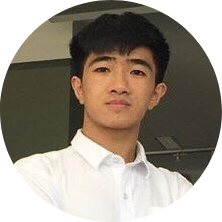
\includegraphics[width=4cm]{profile-modified.png}
    \end{minipage}
    \begin{minipage}{15cm}
        \begin{center}
            \Huge{\textcolor{white}{LE MINH HIEU}} \\
            \vspace*{0.5cm}
            \Large{\textcolor{white}{\textit{Software Developer}}}
        \end{center}
    \end{minipage}
\end{tcolorbox}

\tcbset{colframe=white,colback=white,arc=0mm}
\begin{tcolorbox}
    \begin{minipage}[t]{8cm}
        \vspace*{-0.5cm}
        \begin{tcolorbox}[grow to left by=0.6cm, colback=gray!25,colframe=white]
            \section*{Profiles}
            Passionate embedded software engineer with experience in developing real-time software for a
            range of applications. Involved in the full-life cycle development of several products, my strength
            lies in working co-operatively, remaining flexible and adaptive to changing requirements while remaining
            focused on achieving defined goals. Experienced in working with the Scrum process and finding it to 
            be an effective approach to software development. A dedicated software developer with a track record of
            delivering successful projects.
            
            \section*{Contact}
            \begin{tabular}{r l}
                Tel: & 0366078928 \\
                Email: & minhhieuhcmute@gmail.com \\
                Address: & 299 Lien Phuong street
            \end{tabular}
            
            \section*{Expertise}
            \begin{itemize}
                \item {C/C++}
                \item {OOP design}
                \item {RTOS}
                \item {Linux}
                \item {Bash script}
                \item {Cmake, Make}
                \item {OpenWRT}
                \item {Git}
            \end{itemize}
            
            \section*{Language}
            \begin{itemize}
                \item {Vietnamese: Native Language}
                \item {English: Fluency}
            \end{itemize}
            \vspace*{12\baselineskip}
        \end{tcolorbox}
    \end{minipage}
    \begin{minipage}[t]{11cm}
        \vspace*{-0.5cm}
        \begin{tcolorbox}[grow to right by=0.75cm,colback=white,colframe=white]
            \section*{Education}
            \begin{itemize}
                \item 
                {
                    \textbf{University of technical and education} \\
                    \emph{Bachelor’s degree in Mechatronics Engineering} \\
                    \emph{2014-2018}
                    \begin{itemize}[label=$\circ$]
                        \item {4 consecutive years scholarship rewarded}
                        \item {GPA: 8.3}
                        \item {Top 5 of Teleoperation Water Puppetry Robotic Contest}
                    \end{itemize}
                }
            \end{itemize}

            \section*{Experiences}
            \begin{itemize}
                \item 
                {
                    \textbf{Freelancer} \\
                    \emph{Software Engineer (2022-2024)} \\
                    Working on two based open-source OpenWRT projects:
                    \begin{itemize}[label=$\circ$]
                        \item {Team's size: 2 - Role: Developer}
                        \item {ROOter: https://www.ofmodemsandmen.com/}
                        \item {OpenMPTCP: https://www.openmptcprouter.com/}
                        \item {Add UI web page for the ROOter router}
                        \item {Merge the framework of ROOter and OpenMPTCP together and deploy to a modem hardware}
                        \item {Technical: Lua script, Bash script, network configuration, cross-complilation, Linux (OpenWRT), UI development}
                    \end{itemize}
                }
                \item
                {
                    \textbf{FPT - Outsourcing for Vinfast} \\
                    \emph{Software Engineer (2021-2022)}
                    \begin{itemize}[label=$\circ$]
                        \item {Team's size: 3 - Role: Developer}
                        \item {Deploy \textit{Emergency Call} feature for Vinfast automobile: VFe34, VFe35}
                        \item {Maintain \textit{Backup Battery Management} feature}
                        \item {Contribute to successfully pass the European Homologation}
                        \item {Technical: C/C++, OOP, Make, CMake, Quectel driver, Linux, SELinux, Android Binder}
                    \end{itemize}
                }
                \item 
                {
                    \textbf{Datalogic} \\
                    \emph{Software Engineer (2018-2021)}
                    \begin{itemize}[label=$\circ$]
                        \item {Team's size: 5 - Role: Developer}
                        \item {Add new features to the existing tool that generate configurations for company's products}
                        \item {Design and develop automated unit, component and system tests in 
                        parallel with product software development}
                        \item {Participate in the entire development process of the organization's main products: 
                        \textit{Multi Base Charger, Handheld Scanner}}
                        \item {Study Linux and training for team. Preparing for develop new product which run on Linux instead of RTOS}
                        \item {Technical: C/C++, OOP, design pattern, CMake, RTOS, booting software technique}
                    \end{itemize}
                }
            \end{itemize}
        \end{tcolorbox}
    \end{minipage}

\end{tcolorbox}

\end{document}